\documentclass[tikz,border=9pt]{standalone}
\usepackage{amsmath,amssymb}
\usetikzlibrary{arrows.meta,positioning,calc}
\begin{document}
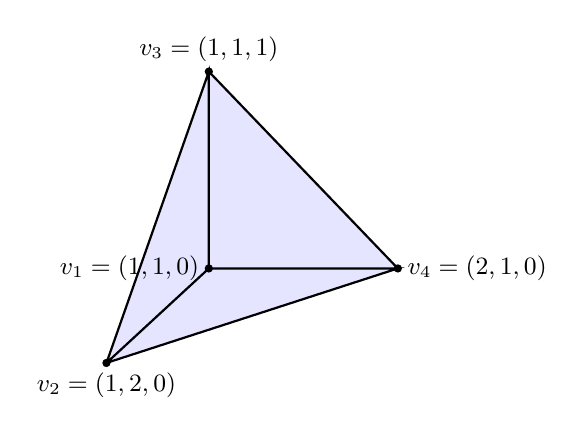
\begin{tikzpicture}[font=\small,arr/.style={-{Stealth},thick},box/.style={draw=blue!55!black,rounded corners,fill=blue!4,align=center,text width=2.9cm,minimum height=1.05cm}]
\begin{scope}[x={(1.2cm,0cm)},y={(-.65cm,-.6cm)},z={(0cm,1.25cm)}]
\coordinate (a) at (0,0,0);\coordinate (b) at (0,2,0);\coordinate (c) at (0,0,2);\coordinate (d) at (2,0,0);
\fill[blue!10] (b)--(c)--(d)--cycle;
\draw[thick] (a)--(b)--(c)--(a)--(d)--(b);\draw[thick] (c)--(d);
\fill (a) circle(1.5pt) node[left]{$v_1=(1,1,0)$};
\fill (b) circle(1.5pt) node[below]{$v_2=(1,2,0)$};
\fill (c) circle(1.5pt) node[above]{$v_3=(1,1,1)$};
\fill (d) circle(1.5pt) node[right]{$v_4=(2,1,0)$};
\end{scope}
\end{tikzpicture}
\end{document}
